% ========================================
%	Header einbinden
% ========================================

\documentclass[bibtotoc,titlepage]{scrartcl}

% Deutsche Spracheinstellungen
\usepackage[ngerman,german]{babel, varioref}
\usepackage[T1]{fontenc}
\usepackage[utf8]{inputenc}

%\usepackage{marvosym}

\usepackage{amsfonts}
\usepackage{amssymb}
\usepackage{amsmath}
\usepackage{amscd}
\usepackage{amstext}

\usepackage{longtable}

%\usepackage{bibgerm}

\usepackage{footnpag}

\usepackage{ifthen}                 %%% package for conditionals in TeX
\usepackage[amssymb]{SIunits}
%Für textumflossene Bilder und Tablellen
%\usepackage{floatflt} - veraltet

%Für Testzwecke aktivieren, zeigt labels und refs im Text an.
%\usepackage{showkeys}

% Abstand zwischen zwei Absätzen nach DIN (1,5 Zeilen)
% \setlength{\parskip}{1.5ex plus0.5ex minus0.5ex}

% Einrückung am Anfang eines neuen Absatzes nach DIN (keine)
%\setlength{\parindent}{0pt}

% Ränder definieren
% \setlength{\oddsidemargin}{0.3cm}
% \setlength{\textwidth}{15.6cm}

% bessere Bildunterschriften
%\usepackage[center]{caption2}


% Problemlösungen beim Umgang mit Gleitumgebungen
\usepackage{float}

% Nummeriert bis zur Strukturstufe 3 (also <section>, <subsection> und <subsubsection>)
%\setcounter{secnumdepth}{3}

% Führt das Inhaltsverzeichnis bis zur Strukturstufe 3
%\setcounter{tocdepth}{3}
\usepackage[version=3]{mhchem}
	\mhchemoptions{minus-sidebearing-left=0.06em, minus-sidebearing-right=0.11em}
\usepackage{exscale}

\newenvironment{dsm} {\begin{displaymath}} {\end{displaymath}}
\newenvironment{vars} {\begin{center}\scriptsize} {\normalsize \end{center}}


\newcommand {\en} {\varepsilon_0}               % Epsilon-Null aus der Elektrodynamik
\newcommand {\lap} {\; \mathbf{\Delta}}         % Laplace-Operator
\newcommand {\R} { \mathbb{R} }                 % Menge der reellen Zahlen
\newcommand {\e} { \ \mathbf{e} }               % Eulersche Zahl
\renewcommand {\i} { \mathbf{i} }               % komplexe Zahl i
\newcommand {\N} { \mathbb{N} }                 % Menge der nat. Zahlen
\newcommand {\C} { \mathbb{C} }                 % Menge der kompl. Zahlen
\newcommand {\Z} { \mathbb{Z} }                 % Menge der kompl. Zahlen
\newcommand {\limi}[1]{\lim_{#1 \rightarrow \infty}} % Limes unendlich
\newcommand {\sumi}[1]{\sum_{#1=0}^\infty}
\newcommand {\rot} {\; \mathrm{rot} \,}         % Rotation
\newcommand {\grad} {\; \mathrm{grad} \,}       % Gradient
\newcommand {\dive} {\; \mathrm{div} \,}        % Divergenz
\newcommand {\dx} {\; \mathrm{d} }              % Differential d
\newcommand {\cotanh} {\; \mathrm{cotanh} \,}   %Cotangenshyperbolicus
\newcommand {\asinh} {\; \mathrm{areasinh} \,}  %Area-Sinus-Hyp.
\newcommand {\acosh} {\; \mathrm{areacosh} \,}  %Area-Cosinus-H.
\newcommand {\atanh} {\; \mathrm{areatanh} \,}  %Area Tangens-H.
\newcommand {\acoth} {\; \mathrm{areacoth} \,}  % Area-cotangens
\newcommand {\Sp} {\; \mathrm{Sp} \,}
\newcommand {\mbe} {\stackrel{\text{!}}{=}}     %Must Be Equal
\newcommand{\qed} { \hfill $\square$\\}
\renewcommand{\i} {\imath}
\def\captionsngerman{\def\figurename{\textbf{Abb.}}}

%%%%%%%%%%%%%%%%%%%%%%%%%%%%%%%%%%%%%%%%%%%%%%%%%%%%%%%%%%%%%%%%%%%%%%%%%%%%
% SWITCH FOR PDFLATEX or LATEX
%%%%%%%%%%%%%%%%%%%%%%%%%%%%%%%%%%%%%%%%%%%%%%%%%%%%%%%%%%%%%%%%%%%%%%%%%%%%
%%%
\ifx\pdfoutput\undefined %%%%%%%%%%%%%%%%%%%%%%%%%%%%%%%%%%%%%%%%% LATEX %%%
%%%
\usepackage[dvips]{graphicx}       %%% graphics for dvips
\DeclareGraphicsExtensions{.eps,.ps}   %%% standard extension for included graphics
\usepackage[ps2pdf]{thumbpdf}      %%% thumbnails for ps2pdf
\usepackage[ps2pdf,                %%% hyper-references for ps2pdf
bookmarks=true,%                   %%% generate bookmarks ...
bookmarksnumbered=true,%           %%% ... with numbers
hypertexnames=false,%              %%% needed for correct links to figures !!!
breaklinks=true,%                  %%% breaks lines, but links are very small
linkbordercolor={0 0 1},%          %%% blue frames around links
pdfborder={0 0 112.0}]{hyperref}%  %%% border-width of frames
%                                      will be multiplied with 0.009 by ps2pdf
%
\hypersetup{ pdfauthor   = {Hannes Franke; Julius Tilly},
pdftitle    = {V301 Innenwiderstand und Leistungsanpassung}, pdfsubject  = {Protokoll FP}, pdfkeywords = {V301, Innenwiderstand, Leistungsanpassung},
pdfcreator  = {LaTeX with hyperref package}, pdfproducer = {dvips
+ ps2pdf} }
%%%
\else %%%%%%%%%%%%%%%%%%%%%%%%%%%%%%%%%%%%%%%%%%%%%%%%%%%%%%%%%% PDFLATEX %%%
%%%
\usepackage[pdftex]{graphicx}      %%% graphics for pdfLaTeX
\DeclareGraphicsExtensions{.pdf}   %%% standard extension for included graphics
\usepackage[pdftex]{thumbpdf}      %%% thumbnails for pdflatex
\usepackage[pdftex,                %%% hyper-references for pdflatex
bookmarks=true,%                   %%% generate bookmarks ...
bookmarksnumbered=true,%           %%% ... with numbers
hypertexnames=false,%              %%% needed for correct links to figures !!!
breaklinks=true,%                  %%% break links if exceeding a single line
linkbordercolor={0 0 1},
linktocpage]{hyperref} %%% blue frames around links
%                                  %%% pdfborder={0 0 1} is the default
\hypersetup{
pdftitle    = {V301 Innenwiderstand und Leistungsanpassung}, 
pdfsubject  = {Protokoll AP}, 
pdfkeywords = {V301, Innenwiderstand, Leistungsanpassung},
pdfsubject  = {Protokoll AP},
pdfkeywords = {V301, Innenwiderstand, Leistungsanpassung}}
%                                  %%% pdfcreator, pdfproducer,
%                                      and CreationDate are automatically set
%                                      by pdflatex !!!
\pdfadjustspacing=1                %%% force LaTeX-like character spacing
\usepackage{epstopdf}
%
\fi %%%%%%%%%%%%%%%%%%%%%%%%%%%%%%%%%%%%%%%%%%%%%%%%%%% END OF CONDITION %%%
%%%%%%%%%%%%%%%%%%%%%%%%%%%%%%%%%%%%%%%%%%%%%%%%%%%%%%%%%%%%%%%%%%%%%%%%%%%%
% seitliche Tabellen und Abbildungen
%\usepackage{rotating}
\usepackage{ae}
\usepackage{
  array,
  booktabs,
  dcolumn
}
\makeatletter 
  \renewenvironment{figure}[1][] {% 
    \ifthenelse{\equal{#1}{}}{% 
      \@float{figure} 
    }{% 
      \@float{figure}[#1]% 
    }% 
    \centering 
  }{% 
    \end@float 
  } 
  \makeatother 


  \makeatletter 
  \renewenvironment{table}[1][] {% 
    \ifthenelse{\equal{#1}{}}{% 
      \@float{table} 
    }{% 
      \@float{table}[#1]% 
    }% 
    \centering 
  }{% 
    \end@float 
  } 
  \makeatother 
%\usepackage{listings}
%\lstloadlanguages{[Visual]Basic}
%\allowdisplaybreaks[1]
%\usepackage{hycap}
%\usepackage{fancyunits}


% ========================================
%	Angaben für das Titelblatt
% ========================================

\title{Versuch 402 - Dispersionsmessung am Glasprisma\\				% Titel des Versuchs 
\large TU Dortmund, Fakultät Physik\\ 
\normalsize Anfänger-Praktikum}

\author{Jan Adam\\			% Name Praktikumspartner A
{\small \href{jan.adam@tu-dortmund.de}{jan.adam@tu-dortmund.de}}	% Erzeugt interaktiven einen Link
\and						% um einen weiteren Author hinzuzfügen
Dimitrios Skodras\\					% Name Praktikumspartner B
{\small \href{dimitrios.skodras@tu-dortmund.de}{dimitrios.skodras@tu-dortmund.de}}		% Erzeugt interaktiven einen Link
}
\date{28.Mai 2013}				% Das Datum der Versuchsdurchführung

% ========================================
%	Das Dokument beginnt
% ========================================

\begin{document}

% ========================================
%	Titelblatt erzeugen
% ========================================

\maketitle					% Jetzt wird die Titelseite erzeugt
\thispagestyle{empty} 				% Weder Kopfzeile noch Fußzeile

% ========================================
%	Der Vorspann
% ========================================

%\newpage					% Wenn Verzeichnisse auf einer neuen Seite beginnen sollen
%\pagestyle{empty}				% Weder Kopf- noch Fußzeile für Verzeichnisse

\tableofcontents

%\newpage					% eine neue Seite
%\thispagestyle{empty}				% Weder Kopf- noch Fußzeile für Verzeichnisse
%\listoffigures					% Abbildungsverzeichnis

%\newpage					% eine neue Seite
%\thispagestyle{empty}				% Weder Kopf- noch Fußzeile für Verzeichnisse
%\listoftables					% Tabellenverzeichnis
\newpage					% eine neue Seite


% ========================================
%	Kapitel
% ========================================

\section{Einleitung}				% Bei Bedarf
\setcounter{page}{1}
Aufgrund der Wechselwirkung von Elektronen in Materie und einfallenden Lichtwellen, ist die Lichtgeschwindigkeit im Medium $v$ geringer als
Die Vakuumlichtgeschwindigkeit $c_0$. Die Brechung von Lichtstrahlen wir durch den Brechungsindex beschrieben, der aus dem Verhältnis der
jeweiligen Lichtgeschwindigkeiten bestimmt wird.
\begin{align}
 n = \frac{v_1}{v_2}
\end{align}
Im Folgenden wird gezeigt, dass die Ausbreitungsgeschwindigkeit und damit der Brechungsindex von der Lichtfrequenz abhängt. Dieses Phänomen
nennt man Dispersion. Im Zuge des Experiments wird das Dispersionsverhalten eines Glasprismas mit Licht des sichtbaren Sprektrums untersucht.
\section{Theorie}
\subsection{Grundlagen der geometrischen Optik}
Wenn ein Lichtstrahl unter einem Winkel $\alpha$ auf eine Grenzschicht zweier Medien auftrifft, wird er gebrochen und breitet sich nun
in einem Winkel $\beta$ gegen die Grenzflächennormale aus. Mithilfe des Huygensschen Prinzips kann der Zusammenhang zwischen den Winkeln
und den Ausbreitungsgeschwindigkeiten berechnet werden. Im Einzelnen lautet es:
\begin{quotation}
 \textit{Jeder Punkt einer bestehenden Wellenfläche kann als Zentrum einer neuen kugelförmigen ``Elementarwelle'' aufgefasst werden. Die Einhüllende aller Elementarwellen gibt die Wellenfront für einen späteren Zeitpunkt an.}
\end{quotation}
\begin{figure}[H]
 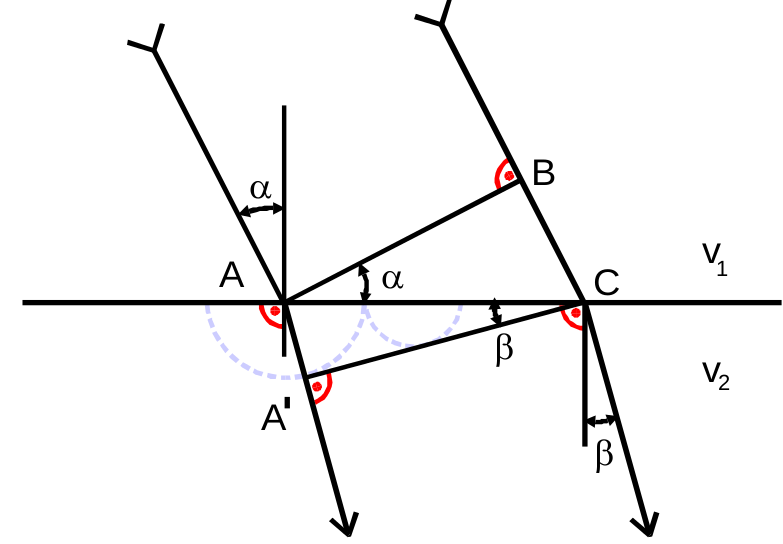
\includegraphics[width=0.7\textwidth]{pics/brechung.png}
 \caption{Brechung zweier paralleler Lichtstrahlen $^{[1]}$}
 \label{pic_snellius}
\end{figure}
Unter Betrachtung von Abbildung \ref{pic_snellius} kann das Verhältnis durch eine Formel ausgedrückt werden. Da der Strahl bei $B$ später
ankommt als bei $A$, ist die Wellenfront bereits um $T\cdot v_2$ ausgedehnt, hingegen bei $C$ noch gar nicht. Aus den Streckenbetrachtungen
der entstehenden einhüllenden Wellenfront ergibt sich das Snelliussche Brechungsgesetz zu
\begin{align}
 \frac{\sin \alpha}{\sin \beta} = \frac{v_1}{v_2}.
 \label{eq_snellius}
\end{align}
\subsection{Dispersionsgleichung}
Leider trifft \eqref{eq_snellius} keine Aussage über die Abhängigkeit zwischen dem Brechungsindex und der Wellenlänge $\lambda$. Um sie
zu finden, wird das Medium auf atomarer Ebene betrachtet. Die elektromagnetische Lichtwelle regt das Elektron zu Schwingungen an. Daher gibt
es eine mediumsabhängige Resonanzfrequenz, bei der die Elektronen merklich Energie absorbieren. Bei Glas ist dies bei sichtbarem Licht nicht
gegeben. Neben der periodischen Anregung $F_e$ durch das Licht, kommen zusätzlich noch die in die Gleichgewichtslage wirkende Kraft $F_r$, sowie
die Dämpfungskräfte $F_d$, die die Bewegung des Elektrons beeinflussen. Somit entsteht folgende Differenzialgleichung
\begin{align}
 m \frac{\dx^2}{\dx t^2}\vec{x} + \vec{F_r} + \vec{F_d} = q \vec{E_0} \e^{i\omega t}
 \label{eq_dgl}
\end{align}
Aus ihrer Lösung entnimmt man die Polarisation eines Mediums, welche mit der Dielektrizitätskonstante $\epsilon$ verknüpft ist. Über die
Maxwellsche Relation
\begin{align}
 \nonumber
 n^2 = \epsilon
\end{align}
lässt sich nun der Zusammenhang zwischen Brechungsindex und Wellelänge ausdrücken. Der daraus entstehende, komplexe Ausdruck wird vereinfacht,
indem nur Wellenlängen benutzt werden, die fern der Resonanzwellenlänge $\lambda_1$ sind. Somit ergeben sich die beiden Dispersionsgleichungen zu
\begin{align}
 &n^2(\lambda) = \sum_{2i=k=0} \frac{A_k}{\lambda ^k} &A_k > 0 \quad \text{für} \quad \lambda \gg \lambda_1 \label{eq_dispgg}\\
 &n^2(\lambda) = 1 - \sum_{2i=k=2} B_k \cdot \lambda^k  &B_k > 0 \quad \text{für} \quad \lambda \ll \lambda_1. \label{eq_displl}
\end{align}
Die zugehörigen Graphen finden sich in Abbildung \ref{pic_dispersion} wieder.
\begin{figure}[H]
 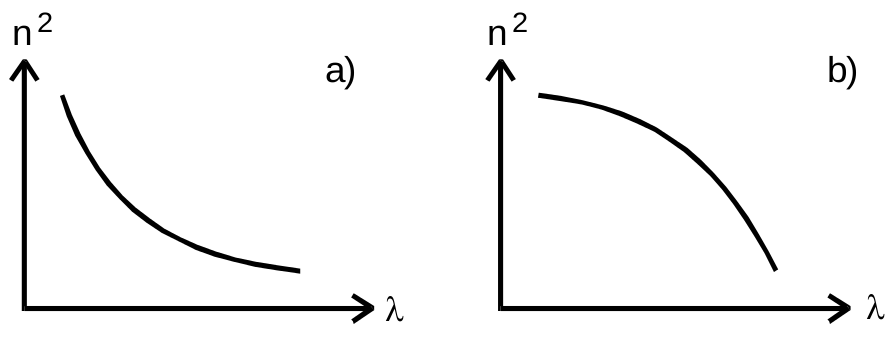
\includegraphics[width= 0.5\textwidth]{pics/dispersion.png}
 \caption{Dispersionskurven nach \eqref{eq_dispgg} für a, und \eqref{eq_displl} für b,}
 \label{pic_dispersion}
\end{figure}

\subsection{Auflösungsvermögen}
Das Auflösungsvermögen ist definiert als:
\begin{align}
	A := \frac{\lambda}{\Delta\lambda}
	\label{eq_resolution2}
\end{align}
Wobei $\lambda$ das Mittel der Wellenlängen zweier Spektrallinien ist, die gerade noch aufgelöst werden können und $\Delta\lambda$ der Wellenlängenunterschied dieser Spektrallinien ist.
Dabei wird das Auflösungsvermögen des Prismas vor allem durch Beugungserscheinungen limitiert. Man kann zwei Spektrallinien genau dann unterscheiden, wenn das Helligkeitsmaximum der einen genau im Helligkeitsminimum der andernen liegt.
Durch einsetzen von Winkelbeziehungen und Näherung für kleine Brechungswinkel $\eta$ ergibt sich aus \eqref{eq_resolution2}
\begin{align}
A = \frac{\lambda}{\Delta\lambda} = b\frac{\text{d}n}{\text{d}\lambda}
\label{eq_resolution}
\end{align}
mit $b =$ Basisbreite des Prismas.

\section{Durchführung}
Die Messungen erfolgen mit Hilfe eines Spektralapparats (Abb.\ref{pic_aufbau}).Die Apparatur besteht aus einem festen Kollimatorrohr, 
welches direkt auf die Lichtquelle ausgerichtet ist, dem Glasprisma, welches auf dem Goniometer verankert ist, und einem schwenkbarem 
Fernrohr. Um scharfe Spektrallinien zu erhalten kann am Kollimatorrohr die Spaltbreite eingestellt werden. Im Fernrohr ist ein 
Fadenkreuz zu sehen, welches auf die Spektrallinien ausgerichtet wird. Das Prisma ist ebenfalls beliebig drehbar. Das Licht verläuft wie 
in Abbildung \ref{pic_aufbau} angedeutet durch den Spalt, wird durch eine Sammellinse parallel auf den Prisma geworfen und dort gebrochen. 
Das gebrochene Licht lässt sich mit dem Fernrohr betrachten.
\begin{figure}[H]
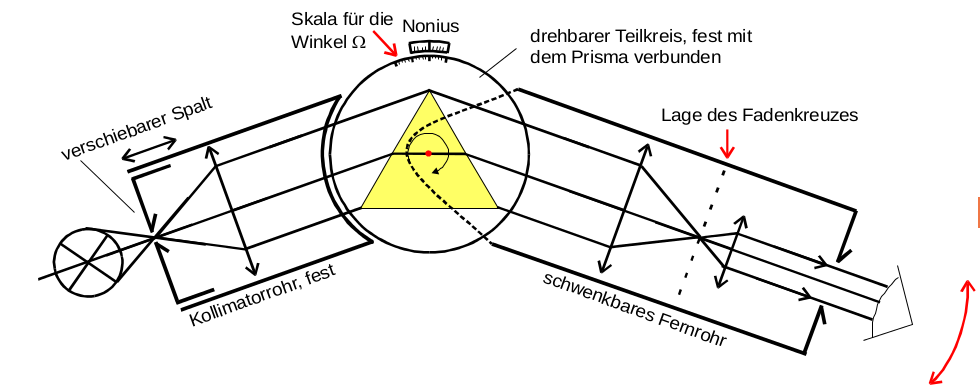
\includegraphics[width=0.8\textwidth]{pics/spek_app.png}
\caption{Aufbau der Messapparatur}
\label{pic_aufbau}
\end{figure}
Um den Brechungsindex in Abhängigkeit von der Wellenlänge $\lambda$ zu bestimmen benötigt man die Winkel $\varphi$ und $\eta$. 
Mit dem Snelliussche Brechungsgesetz und Abbildung \ref{pic_brechung} ergibt sich
\begin{align}
n(\lambda)=\frac{\sin\frac{\eta +\varphi}{2}}{\sin\frac{\varphi}{2}}.
\label{eq_brechung}
\end{align}
\begin{figure}[H]
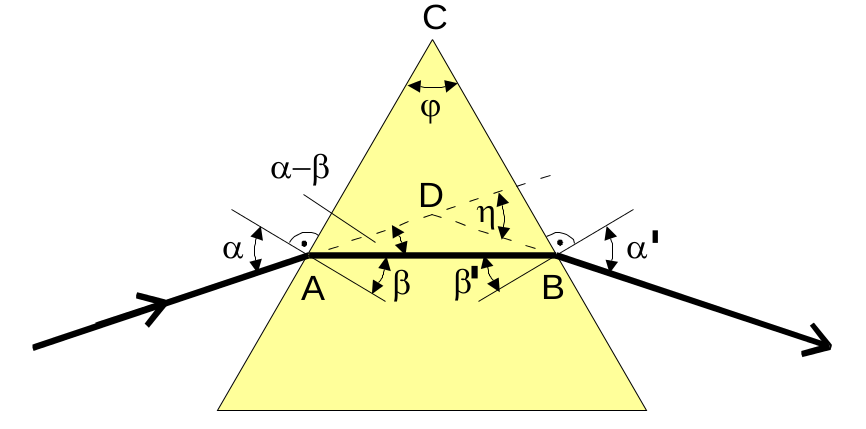
\includegraphics[width=0.5\textwidth]{pics/prisma_sym.png}
\caption{Brechung am Prisma}
\label{pic_brechung}
\end{figure}
Es wird der Spezialfall $\alpha=\alpha^{\prime}$ und $\beta = \beta^{\prime}$ betrachtet um die Bestimmung von $\eta$ und $\varphi$ zu 
vereinfachen.

\subsection{Bestimmung des Prismainnenwinkels $\varphi$}
Um $\varphi$ zu bestimmen wird das Prisma mit der zu messenden Spitze A in Richtung des einfallenden Lichtstrahls ausgerichtet. 
(vgl. Abb.\ref{pic_prismaphi})
\begin{figure}[H]
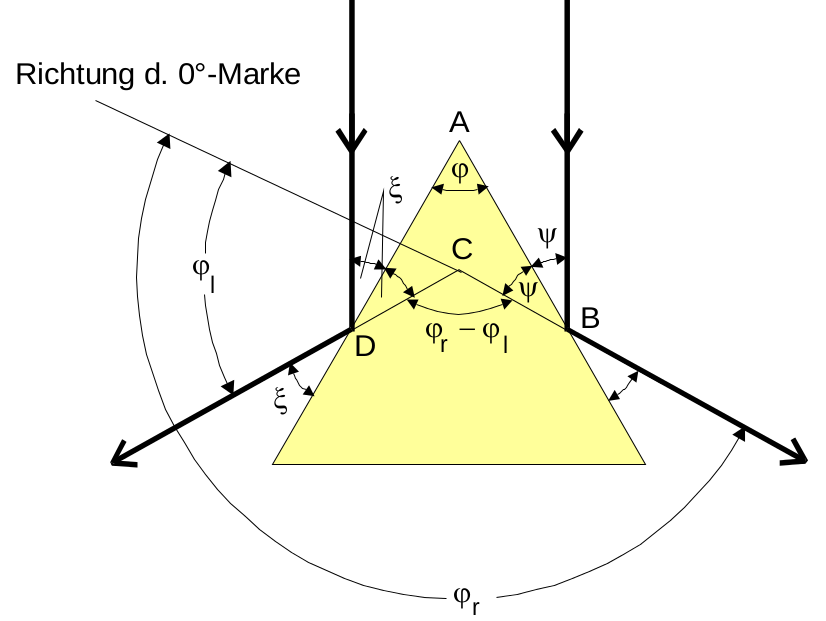
\includegraphics[width=0.6\textwidth]{pics/prisma_phi.png}
\caption{Innenwinkelbestimmung des Prismas}
\label{pic_prismaphi}
\end{figure}
Es müssen wie in Abbildung \ref{pic_prismaphi} zu erkennen die zwei Winkel $\varphi_l$ und $\varphi_r$ gemessen werden. Es gilt dann:
\begin{align}
\varphi=\frac{\varphi_r-\varphi_l}{2}.
\label{eq_phi}
\end{align}
\subsection{Bestimmung des Ablenkungswinkels $\eta$}	
Bei dem Winkel $\eta$ handelt es sich um Richtungsänderungswinkel des eingehenden Strahls. Um diesen mit \eqref{eq_brechung} bestimmen 
zu können, muss der Strahlengang symmetrisch sein,d.h. der gebrochene und der reflektierte Strahl sind parallel. Um diese Vorraussetzung 
zu erfüllen muss das Prisma so ausgerichtet werden, dass das Spaltbild mit dem reflektierten Strahl zusammenfällt. In Abbildung 
\ref{pic_prismaeta} bedeutet das: $\gamma=\gamma^{\prime}=\delta=\delta^{\prime}$.
\begin{figure}[H]
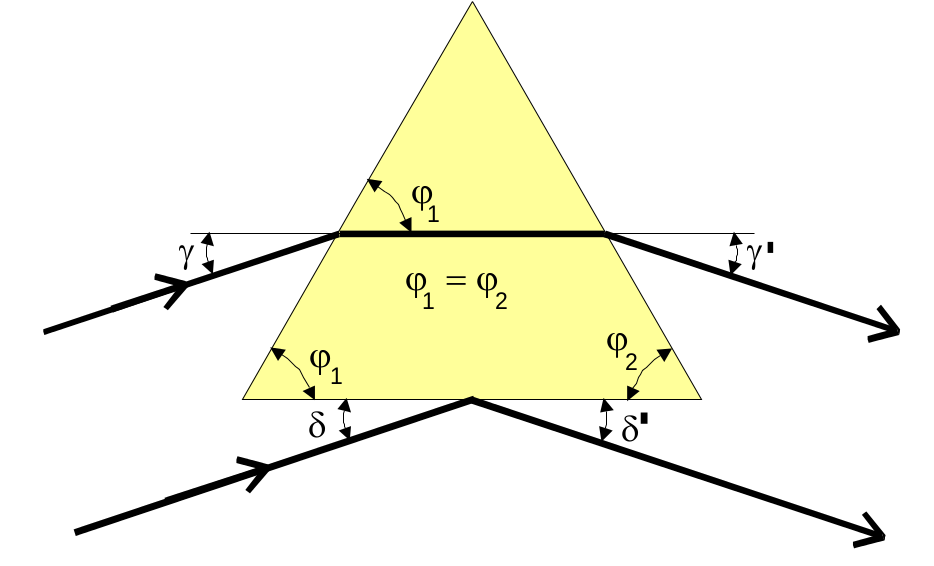
\includegraphics[width=0.6\textwidth]{pics/prisma_eta.png}
\caption{Reflektierter und gebrochener Strahl}
\label{pic_prismaeta}
\end{figure}
Nun werden die Winkel $\Omega_l$ und$\Omega _r$ bestimmt indem das Prisma zunächst wie oben beschrieben ausgerichtet wird und anschließend die Messung in spiegelsymmetrischer Stellung des Prismas durchgeführt wird. Der Winkel ist am Nonius ablesbar.
Die zwei Stellungen des Prismas sind in Abbildung \ref{pic:prisma_etasym} erkennbar.
\begin{figure}[H]
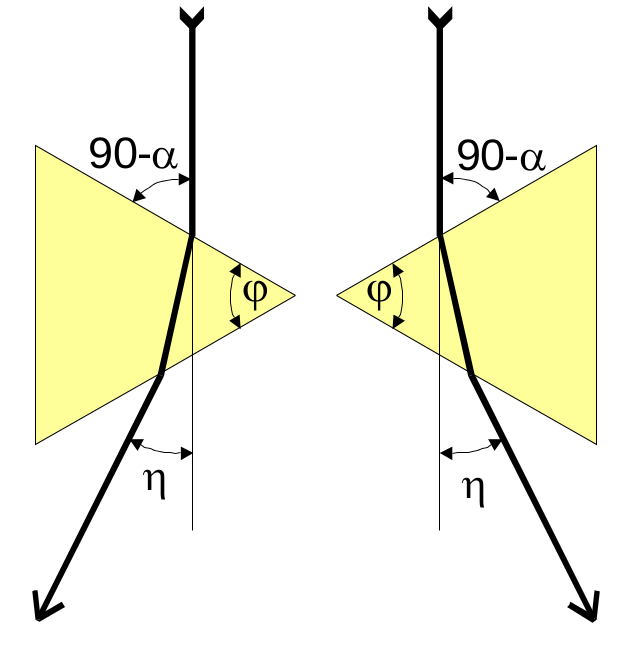
\includegraphics[width=0.3\textwidth]{pics/prisma_ohm.png}
\caption{Spiegelsymmetrische Anordnung des Prismas zur Bestimmung von $\eta$}
\label{pic:prisma_etasym}
\end{figure}
In Abbildung \ref{pic:prisma_ohmlr} sind die Winkelgrößen $\Omega_l$, $\Omega_r$ und die Prismaanordnung erkennbar. 
Der Winkel $\eta$ erechnet sich aus
\begin{align}
\eta = 180 -(\Omega_r-\Omega_l).
\label{eq:eta_ohm_rl}
\end{align}
	
\begin{figure}[H]
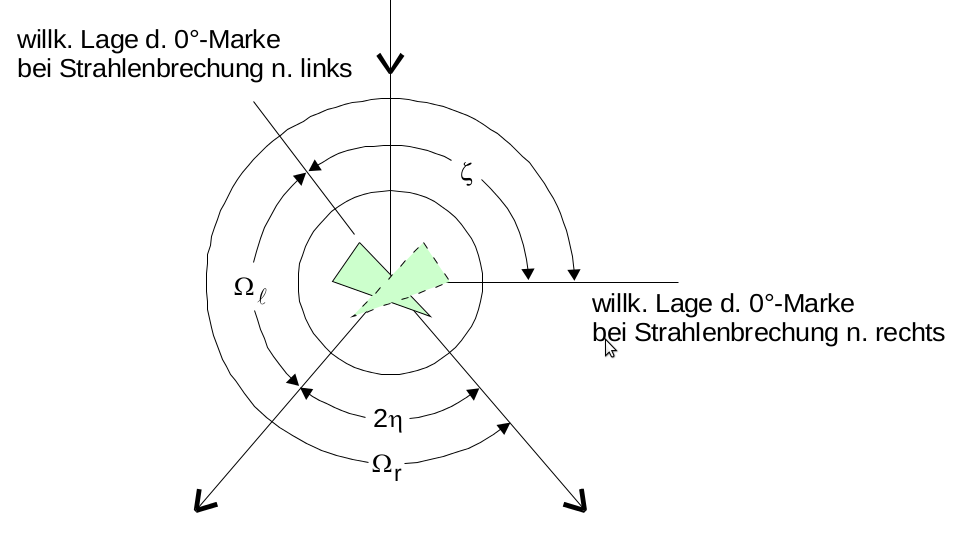
\includegraphics[width=0.7\textwidth]{pics/prisma_ohm1.png}
\caption{Winkel $\Omega_r$ und $\Omega_l$ bezüglich der symmetrischen Anordnung des Prismas}
\label{pic:prisma_ohmlr}
\end{figure}
	 

\section{Auswertung}

\section{Diskussion}


% ========================================
%	Literaturverzeichnis
% ========================================

%\bibliographystyle{plainnat}			% Bibliographie-Style auswählen
%\bibliography{BIBDATEI}			% Literaturverzeichnis

% ========================================
%	Das Dokument endent
% ========================================
\parskip 50pt
\Large{Literatur}\\\\
\large{[1] Versuchsanleitung - Dispersionsmessung am Glasprisma}\\\\
\end{document}
